\documentclass[12pt]{article}
\usepackage[margin=1in]{geometry} 
\usepackage{graphicx}
\usepackage{amsmath,amsthm,amssymb}
\usepackage{hyperref}

\title{
    \textbf{Quiz Assignment} \\ 
    \textbf{MS5033} \\
}

\author{
    \textbf{Darpan Gaur} \\
    \textbf{CO21BTECH11004}
}


\date{}

\begin{document}
\maketitle

\hrulefill

\section*{Problem 1: Variational Derivative of a Functional}
\begin{equation*}\tag{1}
    F[\phi] = \int_{\Omega} [f(\phi, \nabla \phi)] dV 
\end{equation*}
Pertub $\phi$ by $\delta \phi$ such that $\phi \rightarrow \phi + \delta \phi$ and $\nabla \phi \rightarrow \nabla \phi + \nabla \delta \phi$. 
\begin{equation*}\tag{2}
    \begin{split}
        F[\phi + \delta \phi] &= \int_{\Omega} [f(\phi + \delta \phi, \nabla \phi + \nabla \delta \phi)] dV \\
        &= \int_{\Omega} [f(\phi, \nabla \phi) + \delta \phi \frac{\partial f}{\partial \phi} + \nabla \delta \phi \cdot \frac{\partial f}{\partial \nabla \phi}] dV 
    \end{split}
\end{equation*}
Subtracting (1) from (2) we get,
\begin{equation*}\tag{3}
    \begin{split}
        \delta F &= F[\phi + \delta \phi] - F[\phi] \\
        &= \int_{\Omega} [\delta \phi \frac{\partial f}{\partial \phi} + \nabla \delta \phi \cdot \frac{\partial f}{\partial \nabla \phi}] dV
    \end{split}
\end{equation*}
Using integration by parts on the second term in (3),
\begin{equation*}\tag{4}
    \begin{split}
        \delta F &= \int_{\Omega} [\delta \phi \frac{\partial f}{\partial \phi}] dV + [\frac{\partial f}{\partial \nabla \phi} \delta \phi]_{\partial \Omega} - \int_{\Omega} [\nabla \cdot \frac{\partial f}{\partial \nabla \phi} \delta \phi] dV \\ 
        &= \int_{\Omega} [\delta \phi \frac{\partial f}{\partial \phi} - \nabla \cdot \frac{\partial f}{\partial \nabla \phi} \delta \phi] dV \\
        &= \int_{\Omega} [\frac{\partial f}{\partial \phi} - \nabla \cdot \frac{\partial f}{\partial \nabla \phi}] \delta \phi dV
    \end{split}
\end{equation*}
In (4), as $\delta \phi$ is zero at the boundary, the second term vanishes.\\ 
For stationary condition, integral must hold for all variations $\delta \phi$. 
\begin{equation*}\tag{5}
    \boxed{\frac{\partial F}{\partial \phi} = \frac{\partial f}{\partial \phi} - \nabla \cdot \frac{\partial f}{\partial \nabla \phi} }
\end{equation*}

\section*{Problem 2: Functional Derivative of Phase-Field Free Energy}
\subsection*{Part (a)}
\begin{figure}[h]
    \centering
    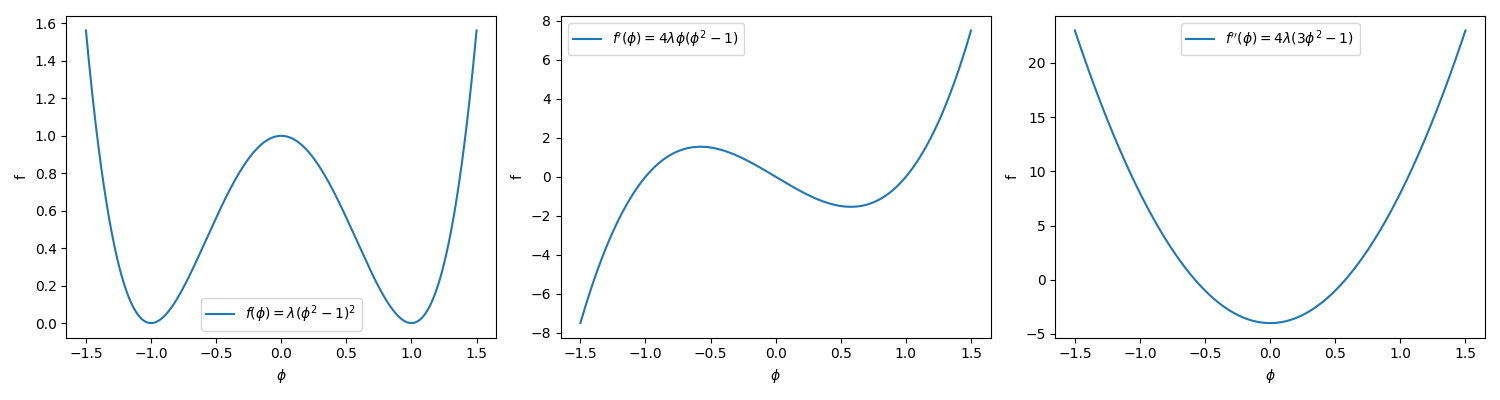
\includegraphics[width=1.0\textwidth]{images/function_sketch.png}
    \caption{Function and its derivatives separately}
\end{figure}
\begin{figure}[h]
    \centering
    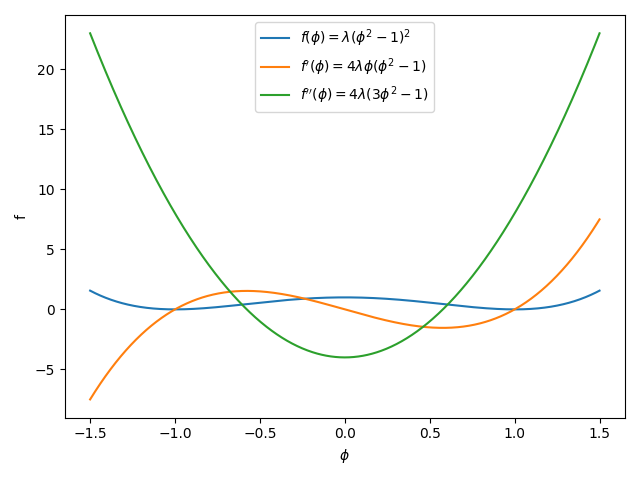
\includegraphics[width=0.6\textwidth]{images/function_sketch_all.png}
    \caption{Function and its derivatives combined}
\end{figure}

\subsection*{Part (b)}
Refer to the python notebook for the code implementation.

\subsection*{Part (c)}
\begin{equation*}
    F[\phi] = \int_{\Omega} [\frac{\kappa}{2} (\nabla \phi)^2 + f(\phi)] dV
\end{equation*}
Here, $f(\phi, \nabla \phi) = \frac{\kappa}{2} (\nabla \phi)^2 + f(\phi)$.\\
We know that,
\begin{equation*}
    \begin{split}
        \frac{\partial F}{\partial \phi} &= \frac{\partial f}{\partial \phi} - \nabla \cdot \frac{\partial f}{\partial \nabla \phi} \\
        &= \frac{\partial f}{\partial \phi} - \nabla \cdot \frac{\partial (\frac{\kappa}{2} (\nabla \phi)^2)}{\partial \nabla \phi} 
    \end{split}
\end{equation*}
\begin{equation*}
    \boxed{\frac{\partial F}{\partial \phi} = \frac{\partial f}{\partial \phi} - \nabla \cdot \kappa \nabla \phi} 
\end{equation*}

\subsection*{Part (d)}
\textbf{$\frac{\partial f}{\partial \phi}$:} local energy density of the phase-field variable $\phi$. Represents phase separation behavior using a double-well potential $f(\phi)$.\\
\\
\textbf{$\nabla \cdot \kappa \nabla \phi$:} Introduces diffusion of the phase-field variable $\phi$ with a diffusivity $\kappa$. Acts as a smoothing term, ensuring that $\phi$ transitions gradually between phases.


\section*{Case Study 1: Derivation of the Cahn-Hillard Equation}
\subsection*{Part (a)}
\begin{equation*}
    F[\phi] = \int_{\Omega} [\frac{\kappa}{2} (\nabla \phi)^2 + f(\phi)] dV
\end{equation*}
Here, $f(\phi, \nabla \phi) = \frac{\kappa}{2} (\nabla \phi)^2 + f(\phi)$.\\
We know that,
\begin{equation*}
    \begin{split}
        \frac{\partial F}{\partial \phi} &= \frac{\partial f}{\partial \phi} - \nabla \cdot \frac{\partial f}{\partial \nabla \phi} \\
        &= \frac{\partial f}{\partial \phi} - \nabla \cdot \frac{\partial (\frac{\kappa}{2} (\nabla \phi)^2)}{\partial \nabla \phi} 
    \end{split}
\end{equation*}
\begin{equation*}
    \boxed{\mu = \frac{\partial F}{\partial \phi} = \frac{\partial f}{\partial \phi} - \nabla \cdot \kappa \nabla \phi} 
\end{equation*}

\subsection*{Part (b)}
By conservative law, 
\begin{equation*}
    \frac{\partial \phi}{\partial t} = \nabla \cdot (M \nabla \mu)
\end{equation*}
\begin{equation*}
    \boxed{\frac{\partial \phi}{\partial t} = \nabla \cdot (M \nabla (\frac{\partial f}{\partial \phi} - \nabla \cdot \kappa \nabla \phi))}
\end{equation*}

\section*{Case Study 2: Boundary Conditions in Cahn-Hillard Equation}
\subsection*{Part (a)}
Consider the Cahn-Hillard equation,
\begin{equation*}
    \frac{\partial \phi}{\partial t} = \nabla \cdot (M \nabla (\frac{\partial f}{\partial \phi} - \nabla \cdot \kappa \nabla \phi))
\end{equation*}
where $F[\phi] = \int_{\Omega} [\frac{\kappa}{2} (\nabla \phi)^2 + f(\phi)] dV$.\\
Variational principle by considering first variation of $F[\phi]$,
\begin{equation*}
    \delta F = \int_{\Omega} [\delta \phi \frac{\partial f}{\partial \phi} - \nabla \cdot \kappa \nabla \delta \phi] dV + \int_{\partial \Omega} [\kappa \nabla \phi \cdot \delta \phi] dS
\end{equation*}
\begin{itemize}
    \item \textbf{No-flux boundary condition}: $n \cdot \nabla \phi = 0$ at $\partial \Omega$. This ensures no transport of $\phi$ across the boundary. As $\mu = \frac{\partial f}{\partial \phi} - \nabla \cdot \kappa \nabla \phi$, imples $\nabla \cdot (\nabla f' - \nabla \cdot \kappa \nabla \phi) = 0$.
    \item \textbf{Dirichlet boundary condition}: $\phi = \phi_0$ at $\partial \Omega$. This ensures a fixed value of $\phi$ at the boundary.
    \item \textbf{Neumann boundary condition}: $\nabla \phi \cdot n = g$ at $\partial \Omega$. This ensures a fixed flux of $\phi$ at the boundary.
    \item \textbf{Periodic boundary condition}: Ensures that $\phi$ and its derivatives repeat across boundaries, often used for systems without explicit boundaries: $\phi(x) = \phi(x + L)$, and $\nabla \phi(x) = \nabla \phi(x + L)$.
\end{itemize}\

\subsection*{Part (b)}
Physical interpretation of the boundary conditions are as follows:
\begin{itemize}
    \item \textbf{No-flux boundary condition}: Used in closed systems where the total amount of $\phi$ is conserved. It ensures that there is no transport of $\phi$ across the boundary ensuring mass conservation.
    \item \textbf{Dirichlet boundary condition}: Used when the value of $\phi$ is known at the boundary. It ensures that the value of $\phi$ is fixed at the boundary. 
    \item \textbf{Neumann boundary condition}: Used when the flux of $\phi$ is known at the boundary. Controls the rate of phase separation at boundaries, often used in systems with external driving forces.
    \item \textbf{Periodic boundary condition}: Used in systems without explicit boundaries. It ensures that the system is translationally invariant, often used in systems with periodic structures.
\end{itemize}

\subsection*{Part (c)}
Periodic boundary conditions are widely used to approximate infinite systems by eliminating boundary effects. 
\begin{itemize}
    \item Seamless continuation of the phase separation process without artificial walls.
    \item Effiecient implementation of Fourier transforms for solving the Cahn-Hilliard equation.
    \item Eliminates the need for explicit boundary conditions, simplifying the problem.
\end{itemize}

\section*{Problem 5: Interpretation of the Cahn-Hillard Equation}
\subsection*{Part (a)}
\textbf{Diffusive term $\nabla \cdot (M \nabla \mu)$}
\begin{itemize}
    \item The diffusive term is responsible for the diffusion of the phase-field variable $\phi$. 
    \item Unlike regular diffusion, the diffusive term includes chemical potential gradient $\nabla \mu$, which drives phase seperation rather than simple concentration gradient.
    \item The diffusive term is proportional to the mobility $M$ and the Laplacian of the chemical potential $\mu$. The Laplacian of the chemical potential $\mu$ is the driving force for the diffusion of the phase-field variable $\phi$. 
\end{itemize} 
\textbf{$\nabla^2 \frac{\partial f}{\partial \phi}$ term}
\begin{itemize}
    \item The higher-order term $-\kappa \nabla^2 \phi$ introduces interfacial effects, penalizing sharp gradients and enforcing a smooth transition between phases.
    \item The bulk free energy density $f(\phi)$ contributes $\frac{\partial f}{\partial \phi}$ dictating the preferred phases.
    \item This term leads to phase separation with surface tension effects, unlike ordinary diffusion which homogenizes concentration.
\end{itemize}

\subsection*{Part (b)}
\begin{itemize}
    \item The diffusion equation leads to smooth spreading of $\phi$, whereas the Cahn-Hilliard equation leads to phase separation and domain formation due to the higher-order derivative term.
    \item Diffusion eqaution uses Flick's second law, whereas Cahn-Hilliard equation uses phase separation dynamics.
    \item The diffusion equation is a linear equation, whereas the Cahn-Hilliard equation is a nonlinear equation.
    \item The Cahn-Hilliard equation ensures conserved dynamics, meaning the total amount of each phase remains fixed, unlike the diffusion equation.
\end{itemize}

\subsection*{Part (c)}
Application of Cahn-Hillard equation are as follows:
\begin{itemize}
    \item \textbf{Image Impainting:} Image inpainting is the filling in of damaged or missing regions of an image with the use of information from surrounding areas.Let f(x), where x = (x, y), be a given binary image in a domain $\Omega$ and $D \subset \Omega$ be the inpainting domain. The image is scaled so that $0 \leq f \leq 1$. Let c(x, t) be a phase-field which is governed by the following modified CH equation:
    \begin{equation*}
        \begin{aligned}
            c_t(x, t) &= \nabla \mu (x, t) + \lambda(f(x)-c(x, t)) \\
            \mu(x, t) &= F' (c(x, t)) - \epsilon^2 \nabla^2 c(x, t), \text{where} F(c) = \frac{1}{4} c^2 (1-c)^2
        \end{aligned}
    \end{equation*} 
    \item \textbf{Tumor Growth Simulation:} To provide optimal strategies for treatments, a mathematical modeling is very useful since it gives systematic investigation. Let $\Omega$ be a computational domain. Let $\Omega_H, \Omega_V, \Omega_D$ be the healthy, viable, and dead tumor tissues, respectively. The Cahn-Hilliard equation naturally captures the evolution of these phases over time, leading to the formation of distinct tumor boundaries.
    \item \textbf{Spinodal Decomposition:} A system of the CH equations is the leading model of spinodal decomposition in binary alloys. Spinodal decomposition is a process by which a mixture of two materials can separate into distinct regions with different material concentrations.
    \item \textbf{Two Phase Fluid Flows:} In the two-phase fluid flow problem, we use the CH equation for capturing the interface location between two immiscible fluids. The CH equation provides a good mass conservation property. We model the variable quantities such as viscosity and density by using the phase-field. Also, we model the surface tension effect with the phase-field. The velocity field is governed by the modified Navier–Stokes equation.
\end{itemize}

\section*{Problem 6: Computing Variational Derivative using SymPy}
Refer to the python notebook for the code implementation.

\end{document}